\subsection{Orthogonal projections}

An important use of the Gram-Schmidt Process is in orthogonal projections, the focus of this section. 

You may recall that a subspace of $\mathbb{R}^n$ is a set of vectors
which contains the zero vector, and is closed under addition and
scalar multiplication. Let's call such a subspace $W$. In particular,
a plane in $\mathbb{R}^n$ which contains the origin, $ \left(0,0,
\cdots, 0 \right)$, is a subspace of $\mathbb{R}^n$.

Suppose a point $Y$ in $\mathbb{R}^n$ is not contained in $W$, then what
point $Z$ in $W$ is closest to $Y$? Using the Gram-Schmidt Process, we
can find such a point. Let $\vect{y}, \vect{z}$ represent the position
vectors of the points $Y$ and $Z$ respectively, with
$\vect{y}-\vect{z}$ representing the vector connecting the two points
$Y$ and $Z$.  It will follow that if $Z$ is the point on $W$ closest
to $Y$, then $\vect{y} - \vect{z}$ will be perpendicular to $W$ (can you see why?); in
other words, $\vect{y} - \vect{z}$ is orthogonal to $W$ (and to every
vector contained in $W$) as in the following diagram.

\begin{center}
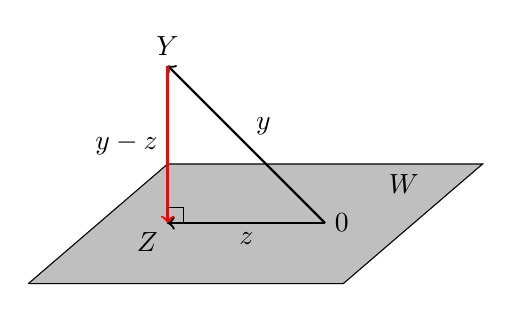
\begin{tikzpicture}
\draw[fill=lightgray](-3,0,2)--(-2,0.75,0)--(2,0.75,0)--(1,0,2)--(-3,0,2);
\draw(-2,0,0) rectangle (-1.8, 0.2,0);
\draw[thick,->](0,0,0)--(-2,0,0);
\draw[thick,->](0,0,0)--(-2,2,0);
\draw[red,thick,->](-2,2,0)--(-2,0,0);
\node[right] at (0,0,0){$0$};
\node[above] at (-2,2,0){$Y$};
\node[below left] at (-2,0,0){$Z$};
\node[below] at (-1,0,0){$\vect{z}$};
\node[above right] at (-1,1,0){$\vect{y}$};
\node[left] at (-2,1,0){$\vect{y}-\vect{z}$};
\node at (1,0.5,0){$W$};
\end{tikzpicture}
\end{center}

The vector $\vect{z}$ is called the \textbf{orthogonal projection} of
$\vec{y}$ on $W$. The definition is given as follows.

\begin{definition}{Orthogonal projection}{orthproj}
Let $W$ be a subspace of $\mathbb{R}^n$, and $Y$ be any point in
$\mathbb{R}^n$. Then the orthogonal projection of $Y$ onto $W$ is given by
\[
\vect{z} = \func{proj}_{W}\left( \vect{y}\right)
=
\left( \frac{\vect{y} \dotprod \vect{w}_1}{ \vectlength \vect{w}_1 \vectlength^2}\right) \vect{w}_1
+
\left( \frac{\vect{y} \dotprod \vect{w}_2}{ \vectlength \vect{w}_2 \vectlength^2}\right) \vect{w}_2
+
\cdots
+
\left( \frac{\vect{y} \dotprod \vect{w}_m}{ \vectlength \vect{w}_m \vectlength^2}\right) \vect{w}_m
\]
where $\{\vect{w}_1, \vect{w}_2, \cdots, \vect{w}_m \}$ is any orthogonal basis of $W$.
\end{definition}

Therefore, in order to find the orthogonal projection, we must first
find an orthogonal basis for the subspace. Note that one could use an
orthonormal basis, but it is not necessary in this case since as you
can see above the normalization of each vector is included in the
formula for the projection.

Before we explore this further through an example, we show that the
orthogonal projection does indeed yield a point $Z$ (the point whose position
vector is the vector $\vect{z}$ above) which is the point of $W$
closest to $Y$.

\begin{theorem}{Approximation theorem}{approximation}
Let $W$ be a subspace of $\mathbb{R}^n$ and $Y$ any point in
$\mathbb{R}^n$. Let $Z$ be the point whose position vector is the
orthogonal projection of $Y$ onto $W$. \\
Then, $Z$ is the point in $W$ closest to $Y$.
\end{theorem}

\begin{proof}
First $Z$ is certainly a point in $W$  since it is in the span of a basis of $W$. 

To show that $Z$ is the point in $W$ closest to $Y$, we wish to show
that $|\vect{y}-\vect{z}_1| > |\vect{y}-\vect{z}|$ for all $\vect{z}_1
\neq \vect{z} \in W$.  We begin by writing $\vect{y}-\vect{z}_1 =
(\vect{y} - \vect{z}) + (\vect{z} -
\vect{z}_1)$.  Now, the vector $\vect{y} - \vect{z}$ is orthogonal to
$W$, and $\vect{z} - \vect{z}_1$ is contained in $W$. Therefore these
vectors are orthogonal to each other. By the Pythagorean Theorem, we
have that
\[
\vectlength \vect{y} - \vect{z}_1 \vectlength^2 = \vectlength \vect{y} - \vect{z}\vectlength ^2 + \vectlength \vect{z} -\vect{z}_1 \vectlength ^2 > \vectlength \vect{y} - \vect{z} \vectlength^2
\]
This follows because $\vect{z} \neq \vect{z}_1$ so
$\vectlength\vect{z} -\vect{z}_1 \vectlength^2 > 0.$

Hence, $\vectlength \vect{y} - \vect{z}_1 \vectlength^2 > \vectlength
\vect{y} - \vect{z} \vectlength^2$. Taking the square root of each
side, we obtain the desired result.
\end{proof}

Consider the following example.

\begin{example}{Orthogonal projection}{orthproj}
Let $W$ be the plane through the origin given by the equation $x - 2y
+ z = 0$. \\
Find the point in $W$ closest to the point $Y = (1,0,3)$.
\end{example}

\begin{solution}
We must first find an orthogonal basis for $W$. Notice that $W$ is
characterized by all points $(a,b,c)$ where $c = 2b-a$. In other
words,
\[
W = 
\leftB
\begin{array}{c}
a \\
b \\
2b - a 
\end{array}
\rightB
= 
a \leftB
\begin{array}{c}
1 \\
0 \\
-1 
\end{array}
\rightB
+ 
b \leftB
\begin{array}{c}
0 \\
1 \\
2 
\end{array}
\rightB, 
\; 
a,b \in \mathbb{R}
\] 

We can thus write $W$ as 
\begin{eqnarray*}
W &=& \mbox{span} \left\{ \vect{u}_1, \vect{u}_2 \right\} \\
 &=& \mbox{span} 
\left\{
\leftB
\begin{array}{r}
1 \\
0 \\
-1
\end{array}
\rightB,
\leftB
\begin{array}{c}
0 \\
1 \\
2
\end{array}
\rightB
\right\}
\end{eqnarray*}

Notice that this span is a basis of $W$ as it is linearly
independent. We will use the Gram-Schmidt Process to convert this to
an orthogonal basis, $\left\{\vect{w}_1, \vect{w}_2 \right\}$. In this
case, as we remarked it is only necessary to find an orthogonal basis, and it is not
required that it be orthonormal.

\[
\vect{w}_1 = \vect{u}_1 = \leftB \begin{array}{r}
1 \\
0 \\
-1
\end{array}
\rightB
\]
\begin{eqnarray*}
\vect{w}_2 &=& \vect{u}_2 - \left(  \frac{ \vect{u}_2 \dotprod \vect{w}_1}{\vectlength \vect{w}_1 \vectlength^2} \right)  \vect{w}_1\\
&=& \leftB
\begin{array}{c}
0 \\
1 \\
2
\end{array}
\rightB
-
\left(
\frac{-2}{2}\right)
\leftB
\begin{array}{r}
1 \\
0 \\
-1
\end{array}
\rightB
\\
&=&
\leftB
\begin{array}{c}
0 \\
1 \\
2
\end{array}
\rightB 
+
\leftB
\begin{array}{r}
1 \\
0 \\
-1
\end{array}
\rightB \\
&=&
\leftB
\begin{array}{c}
1 \\
1 \\
1
\end{array}
\rightB
\end{eqnarray*}

Therefore an orthogonal basis of $W$ is 
\[
\left\{ \vect{w}_1, \vect{w}_2 \right\} = 
\left\{
\leftB \begin{array}{r}
1 \\
0 \\
-1
\end{array}
\rightB, 
\leftB
\begin{array}{c}
1 \\
1 \\
1
\end{array}
\rightB
\right\}
\]

We can now use this basis to find the orthogonal projection of the
point $Y=(1,0,3)$ on the subspace $W$. We will write the position
vector $\vect{y}$ of $Y$ as $\vect{y} = \leftB \begin{array}{c} 1 \\ 0 \\ 3
\end{array} \rightB$. Using Definition \ref{def:orthproj}, we compute the projection as follows:
\begin{eqnarray*}
\vect{z} &=& \func{proj}_{W}\left( \vect{y}\right)\\
&=&
\left( \frac{\vect{y} \dotprod \vect{w}_1}{ \vectlength \vect{w}_1 \vectlength^2}\right) \vect{w}_1
+
\left( \frac{\vect{y} \dotprod \vect{w}_2}{ \vectlength \vect{w}_2 \vectlength^2}\right) \vect{w}_2 \\
&=&
\left( \frac{-2}{2} \right) \leftB
\begin{array}{r}
1 \\
0 \\
-1
\end{array}
\rightB
+
\left( \frac{4}{3} \right)
\leftB
\begin{array}{c}
1 \\
1 \\
1 
\end{array}
\rightB \\
&=& 
\leftB
\begin{array}{c}
\vspace{0.05in}\frac{1}{3} \\
\vspace{0.05in}\frac{4}{3} \\
\vspace{0.05in}\frac{7}{3} 
\end{array}
\rightB
\end{eqnarray*}

Therefore the point $Z$ on $W$ closest to the point $(1,0,3)$  is $\left( \frac{1}{3}, \frac{4}{3}, \frac{7}{3} \right)$. 

\end{solution}

Recall that the vector $\vect{y} - \vect{z}$ is perpendicular
(orthogonal) to all the vectors contained in the plane $W$. Using a
basis for $W$, we can in fact find all such vectors which are
perpendicular to $W$. We call this set of vectors the
\textbf{orthogonal complement}\index{orthogonal complement} of $W$ and
denote it $W^{\perp}$.

\begin{definition}{Orthogonal complement}{orthcomp}
Let $W$ be a subspace of $\mathbb{R}^n$. Then the orthogonal
complement of $W$, written $W^{\perp}$, is the set of all vectors
$\vect{x}$ such that $\vect{x} \dotprod \vect{z} = 0$ for all vectors
$\vect{z}$ in $W$.
\[
W^{\perp} = \{ \vect{x} \in \mathbb{R}^n \; \mbox{such that} \;
\vect{x} \dotprod \vect{z} = 0 \; \mbox{for all} \; \vect{z} \in W \}
\]
\end{definition}

The orthogonal complement is defined as the set of all vectors which are orthogonal to all vectors in the original subspace. It turns out that it is sufficient that the vectors in the orthogonal complement be orthogonal to a spanning set of the original space.

\begin{proposition}{Orthogonal to spanning set}{orthogonalspanningset}
Let $W$ be a subspace of $\mathbb{R}^n$ such that $W = \func{span} \left\{ \vect{w}_1, \vect{w}_2, \cdots, \vect{w}_m \right\}$. Then $W^{\perp}$ is the set of all vectors which are orthogonal to each $\vect{w}_i$ in the spanning set. 
\end{proposition}

The following proposition demonstrates that the orthogonal complement of a subspace is itself a subspace. 

\begin{proposition}{The orthogonal complement}{subspacecomplement}
Let $W$ be a subspace of $\mathbb{R}^n$. Then the orthogonal complement $W^{\perp}$ is also a subspace of $\mathbb{R}^n$.
\end{proposition}

Consider the following proposition.

\begin{proposition}{Orthogonal complement of $\mathbb{R}^n$}{complementofrn}
The complement of $\mathbb{R}^n$ is the set containing the zero vector:
\[
 (\mathbb{R}^n)^{\perp} = \left\{ \vect{0} \right\}
\]
Similarly, 
\[
\left\{ \vect{0} \right\}^{\perp} = (\mathbb{R}^n)
\]
\end{proposition}

\begin{proof}
Here, $\vect{0}$ is the zero vector of $\mathbb{R}^n$.
Since $\vect{x}\dotprod\vect{0}=0$ for all $\vect{x}\in\mathbb{R}^n$, 
$\mathbb{R}^n\subseteq\{ \vect{0}\}^{\perp}$.
Since $\{ \vect{0}\}^{\perp}\subseteq\mathbb{R}^n$, the equality follows,
i.e., $\{ \vect{0}\}^{\perp}=\mathbb{R}^n$.

Again, since $\vect{x}\dotprod\vect{0}=0$ for all $\vect{x}\in\mathbb{R}^n$,
$\vect{0}\in (\mathbb{R}^n)^{\perp}$, so $\{ \vect{0}\}\subseteq(\mathbb{R}^n)^{\perp}$.
Suppose $\vect{x}\in\mathbb{R}^n$, $\vect{x}\neq\vect{0}$.  
Since $\vect{x}\dotprod\vect{x}=||\vect{x}||^2$ and $\vect{x}\neq\vect{0}$,
$\vect{x}\dotprod\vect{x}\neq 0$, so $\vect{x}\not\in(\mathbb{R}^n)^{\perp}$.
Therefore $(\mathbb{R}^n)^{\perp}\subseteq \{\vect{0}\}$, and thus
$(\mathbb{R}^n)^{\perp}=\{\vect{0}\}$.
\end{proof}

In the next example, we will look at how to find
$W^{\perp}$.

\begin{example}{Orthogonal complement}{orthcomp}
Let $W$ be the  plane through the origin given by the equation  $x - 2y + z = 0$. Find
a basis for the orthogonal complement of $W$.
\end{example}

\begin{solution}

From Example \ref{exa:orthproj} we know that we can write $W$ as 
\[
W = \mbox{span} \left\{ \vect{u}_1, \vect{u}_2 \right\} = \mbox{span} 
\left\{
\leftB
\begin{array}{r}
1 \\
0 \\
-1
\end{array}
\rightB,
\leftB
\begin{array}{c}
0 \\
1 \\
2
\end{array}
\rightB
\right\}
\]

In order to find $W^{\perp}$, we need to find all $\vect{x}$ which are orthogonal to every vector in this span. 

Let $\vect{x} = \leftB
\begin{array}{c}
x_1 \\
x_2 \\
x_3
\end{array}
\rightB$. 
In order to satisfy $\vect{x} \dotprod \vect{u}_1 = 0$, the following equation must hold. 
\[
x_1 - x_3 = 0
\]

In order to satisfy $\vect{x} \dotprod \vect{u}_2 = 0$, the following equation must hold.
\[
x_2 + 2x_3 = 0 
\]

Both of these equations must be satisfied, so we have the following system of equations. 
\[
\begin{array}{c}
x_1 - x_3 = 0 \\
x_2 + 2x_3 = 0
\end{array}
\]

To solve, set up the augmented matrix. 

\[
\leftB \begin{array}{rrr|r}
1 & 0 & -1 & 0 \\
0 & 1 & 2 & 0 
\end{array} \rightB
\]

Using Gaussian Elimination, we find that $W^{\perp} = \mbox{span} \left\{ \leftB
\begin{array}{r}
1 \\
-2 \\
1
\end{array}
\rightB
\right\}$, and hence 
$\left\{ \leftB
\begin{array}{r}
1 \\
-2 \\
1
\end{array}
\rightB
\right\}$ is a basis for  $W^{\perp}$. 
\end{solution}

The following results summarize the important properties of the orthogonal projection. 

\begin{theorem}{Orthogonal projection}{orthproj}
Let $W$ be a subspace of $\mathbb{R}^n$, $Y$ be any point in $\mathbb{R}^n$, and let $Z$ be the point in $W$ closest to $Y$. Then, 
\begin{enumerate}
\item 
The position vector $\vect{z}$ of the point $Z$ is given by $\vect{z} = \func{proj}_{W}\left( \vect{y}\right)$
\item
$\vect{z} \in W$ and $\vect{y} - \vect{z} \in W^{\perp}$
\item
$| Y - Z | < | Y - Z_1 |$ for all $Z_1 \neq Z \in W$
\end{enumerate}
\end{theorem}

Consider the following example of this concept.

\begin{example}{Find a vector closest to a given vector}{vectorclosestvector}

Let
\[ \vect{x}_1=\leftB\begin{array}{c} 1\\ 0\\ 1\\ 0 \end{array}\rightB,
\vect{x}_2=\leftB\begin{array}{c} 1\\ 0\\ 1\\ 1 \end{array}\rightB,
\vect{x}_3=\leftB\begin{array}{c} 1\\ 1\\ 0\\ 0 \end{array}\rightB,
\mbox{ and }
\vect{v}=\leftB\begin{array}{c} 4\\ 3\\ -2\\ 5 \end{array}\rightB. \]
We want to find the vector in
$W =\func{span}\{\vect{x}_1, \vect{x}_2,\vect{x}_3\}$
closest to $\vect{y}$.
\end{example}

\begin{solution}
We will first use the Gram-Schmidt Process to construct the orthogonal basis, $B$, of $W$:
\[ B=\left\{
\leftB\begin{array}{c} 1\\ 0\\ 1\\ 0 \end{array}\rightB,
\leftB\begin{array}{c} 0\\ 0\\ 0\\ 1 \end{array}\rightB,
\leftB\begin{array}{r} 1\\ 2\\ -1\\ 0 \end{array}\rightB
\right\}.\]

By Theorem \ref{thm:orthproj},
\[ \func{proj}_U(\vect{v}) = 
\frac{2}{2} \leftB\begin{array}{c} 1\\ 0\\ 1\\ 0 \end{array}\rightB +
\frac{5}{1}\leftB\begin{array}{c} 0\\ 0\\ 0\\ 1 \end{array}\rightB +
\frac{12}{6}\leftB\begin{array}{r} 1\\ 2\\ -1\\ 0 \end{array}\rightB
= \leftB\begin{array}{r} 3\\ 4\\ -1\\ 5 \end{array}\rightB
\]
is the vector in $U$ closest to $\vect{y}$.
\end{solution}

Consider the next example. 

\begin{example}{Vector written as a sum of two vectors}{sumoftwovectors}
Let $W$ be a subspace given by $W = \mbox{span} \left\{
\leftB
\begin{array}{c}
1 \\
0 \\
1 \\
0 \\
\end{array}
\rightB, 
\leftB 
\begin{array}{c}
0 \\
1 \\
0 \\
2 \\
\end{array}
\rightB
\right\}$, and $Y = (1,2,3,4)$. \\
Find the point $Z$ in $W$ closest to $Y$, and moreover write $\vect{y}$ as the sum of a  vector in $W$ and a vector in $W^{\perp}$. 
\end{example}

\begin{solution}
From Theorem \ref{thm:approximation}, the point $Z$ in $W$ closest to
$Y$ is given by $\vect{z} = \func{proj}_{W}\left( \vect{y}\right)$.

Notice that since the above vectors already give an orthogonal basis for $W$, we have:

\begin{eqnarray*}
\vect{z} &=& \func{proj}_{W}\left( \vect{y}\right)\\
&=&
\left( \frac{\vect{y} \dotprod \vect{w}_1}{ \vectlength \vect{w}_1 \vectlength^2}\right) \vect{w}_1
+
\left( \frac{\vect{y} \dotprod \vect{w}_2}{ \vectlength \vect{w}_2 \vectlength^2}\right) \vect{w}_2 \\
&=& 
\left( \frac{4}{2} \right) \leftB
\begin{array}{c}
1 \\
0 \\
1 \\
0 
\end{array}
\rightB
+
\left( \frac{10}{5} \right)
\leftB
\begin{array}{c}
0 \\
1 \\
0 \\
2
\end{array}
\rightB \\
&=& 
\leftB
\begin{array}{c}
2 \\
2 \\
2 \\
4 
\end{array}
\rightB
\end{eqnarray*} 

Therefore the point in $W$ closest to $Y$ is $Z = (2,2,2,4)$. \\

Now, we need to write $\vect{y}$ as the sum of a vector in $W$ and a
vector in $W^{\perp}$. This can easily be done as follows:
\[
\vect{y} = \vect{z} + (\vect{y} - \vect{z})
\]
since $\vect{z}$ is in $W$ and as we have seen $\vect{y} - \vect{z}$ is in  $W^{\perp}$. \\
The vector $\vect{y} - \vect{z}$ is given by 
\[
\vect{y} - \vect{z} = \leftB
\begin{array}{c}
1 \\
2 \\
3 \\
4 
\end{array}
\rightB
-
\leftB
\begin{array}{c}
2 \\
2 \\
2 \\
4 
\end{array}
\rightB
 = 
\leftB
\begin{array}{r}
-1 \\
0 \\
1 \\
0
\end{array}
\rightB
\]
Therefore, we can write $\vect{y}$ as
\[
\leftB
\begin{array}{c}
1 \\
2 \\
3 \\
4 
\end{array}
\rightB
=
\leftB
\begin{array}{c}
2 \\
2 \\
2 \\
4 
\end{array}
\rightB
+
\leftB
\begin{array}{r}
-1 \\
0 \\
1 \\
0
\end{array}
\rightB
\]
\end{solution}

\begin{example}{Point in a plane closest to a given point}{closestplane}
Find the point $Z$ in the plane $3x+y-2z=0$ that is closest to
the point $Y=(1,1,1)$.
\end{example}

\begin{solution}
The solution will proceed as follows.
\begin{enumerate}
\item Find a basis $X$ of the subspace $W$ of $\mathbb{R}^3$ defined by
the equation  $3x+y-2z=0$.
\item Orthogonalize the basis $X$ to get an orthogonal basis
$B$ of $W$.
\item Find the projection on $W$ of the position vector of
the point $Y$.
\end{enumerate}

We now begin the solution.
\begin{enumerate}
\item $3x+y-2z=0$ is a system of one equation in three variables.
Putting the augmented matrix in {\rref}:
\[
\leftB\begin{array}{rrr|r} 3 & 1 & -2 & 0 \end{array}\rightB
\rightarrow
\leftB\begin{array}{rrr|r} 1 & \frac{1}{3} & -\frac{2}{3} & 0 \end{array}\rightB
\]
gives general solution $x=\frac{1}{3}s+\frac{2}{3}t$, $y=s$, $z=t$
for any $s,t\in\mathbb{R}$.
Then  
\[
W=\func{span} \left\{
\leftB\begin{array}{r} -\frac{1}{3} \\ 1 \\ 0 \end{array}\rightB,
\leftB\begin{array}{r} \frac{2}{3} \\ 0 \\ 1 \end{array}\rightB\right\}
\]
Let
$X=\left\{
\leftB\begin{array}{r} -1 \\ 3 \\ 0 \end{array}\rightB,
\leftB\begin{array}{r} 2 \\ 0 \\ 3 \end{array}\rightB\right\}$.
Then $X$ is linearly independent and $\func{span}(X)=W$, so $X$ is a basis of $W$.

\item Use the Gram-Schmidt Process to get an
orthogonal basis of $W$: 


\[ \vect{f}_1=\leftB\begin{array}{r} -1 \\ 3 \\ 0 \end{array}\rightB
\mbox{ and }
\vect{f}_2 =
\leftB\begin{array}{r} 2 \\ 0 \\ 3 \end{array}\rightB
-\frac{-2}{10}\leftB\begin{array}{r} -1 \\ 3 \\ 0 \end{array}\rightB
=\frac{1}{5}\leftB\begin{array}{r} 9 \\ 3 \\ 15 \end{array}\rightB.\]
Therefore
$B=\left\{ \leftB\begin{array}{r} -1 \\ 3 \\ 0 \end{array}\rightB,
\leftB\begin{array}{r} 3 \\ 1 \\ 5 \end{array}\rightB \right\}$ is
an orthogonal basis of $W$.
\item To find 
the point $Z$ on $W$ closest to $Y=(1,1,1)$, compute
\begin{eqnarray*}
\func{proj}_{W}\leftB\begin{array}{r} 1 \\ 1 \\ 1 \end{array}\rightB
& = &
\frac{2}{10} \leftB\begin{array}{r} -1 \\ 3 \\ 0 \end{array}\rightB
+ \frac{9}{35}\leftB\begin{array}{r} 3 \\ 1 \\ 5 \end{array}\rightB\\
& = & 
\frac{1}{7}\leftB\begin{array}{r} 4 \\ 6 \\ 9 \end{array}\rightB.
\end{eqnarray*}
Therefore, $Z=\left( \frac{4}{7}, \frac{6}{7}, \frac{9}{7}\right)$.
\end{enumerate}
\end{solution}
